\title{Лекции по ФИЛП}
\chapter{Лекция 1}--
Lisp - безтиповый язык. Атомы - символы, которые могут обозначать любый объекты. Самовычислительные атомы - T, Nil, числа, строки.\\

Точечная пара - (A.B):\\
$\square \square \rightarrow cdr$\\
$\downarrow$\\
car

Пустая конструкция - () - Nil.

\chapter{Лекция 2}\

\begin{figure}[H]
	\center{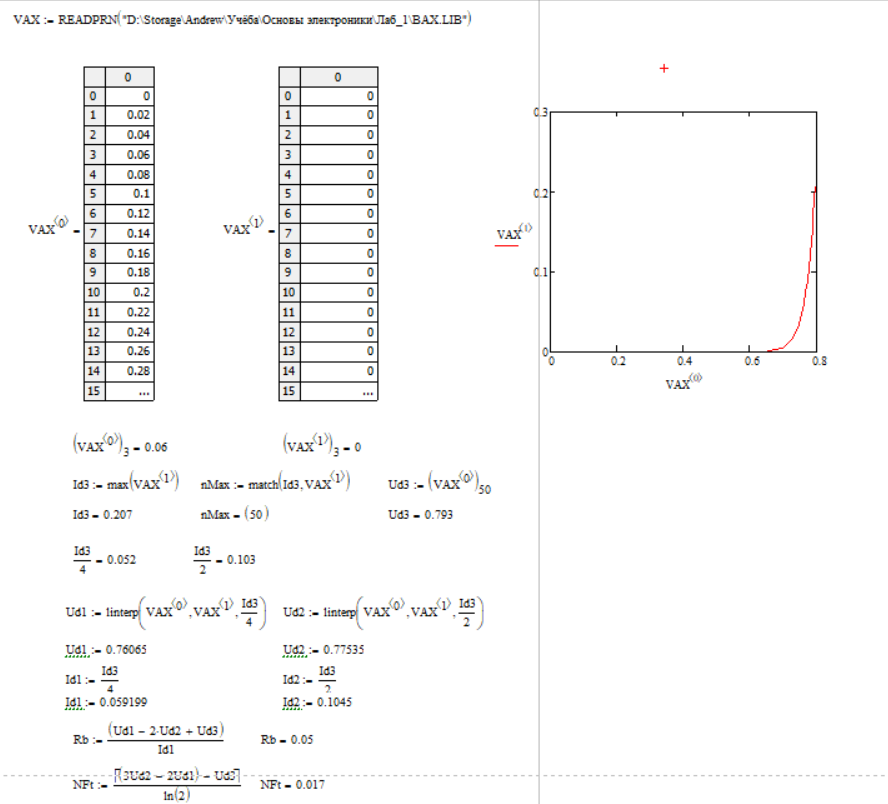
\includegraphics[scale=0.5]{0}}
	\caption{Виды структур в lisp}
\end{figure}

\section{Представление атома в памяти}
Представление атома в памяти - атом представляется в памяти в виде структуры, содержащей пять указателей:
\begin{itemize}
\item name - символьный идентификатор атома
\item value - самоопределяемое значение атома
\item function - лямбда-выражение
\item properties - список свойств
\item package - пакет, указатель на начало области, связывающий значение атома и пространство имён
\end{itemize}

\section{Классификация функций}
\begin{itemize}
\item чистые функции (математические)
\item формы (специальные функции), могут принимать различное число аргументов
\item псевдо-функции (вывод на экран)
\item функции с вариантами значений
\item функционалы - принимают функцию в качестве параметров, либо возвращаемым значением является функция
\item базисные функции - car, cdr, cons, atom, cond, quote, eval, lambda, apply, funcall
\end{itemize}

Выяснить атом - перейти по указателю.

Лямбда-выражение - (lambda (параметры) (тело)).

Вызов: (лямбда-выражение аргументы)

\section{Именованные функции}
Синтаксис:\\
(defun имя лямбда-выражение)\\
(defun f $(x_{1},... x_{k})$ форма)\\

Лямбда-определение может оказаться более эффективным. Пример лямбда-определения:\\
$(let (x_{1} p_{1}) (x_{2} p_{2}) ... (x_{k}  p_{k}) e) = ((lambda (x_{1}, x_{2},... x_{k}) e) p_{1} p_{2} ... p_{k})$\\

\section{Классификация по операциям работы со списку}
1. Селекторы - car, cdr\\
2. Функции-конструкторы - cons, list\\
3. Функции-предикаты - atom, null, listp, consp, eql (eql сравнивает атомы и числа одного типа, применим только к числам) equal (как eql и списки), equalp (equal + "=").

\section{Вычисление функций}
\begin{figure}[H]
	\center{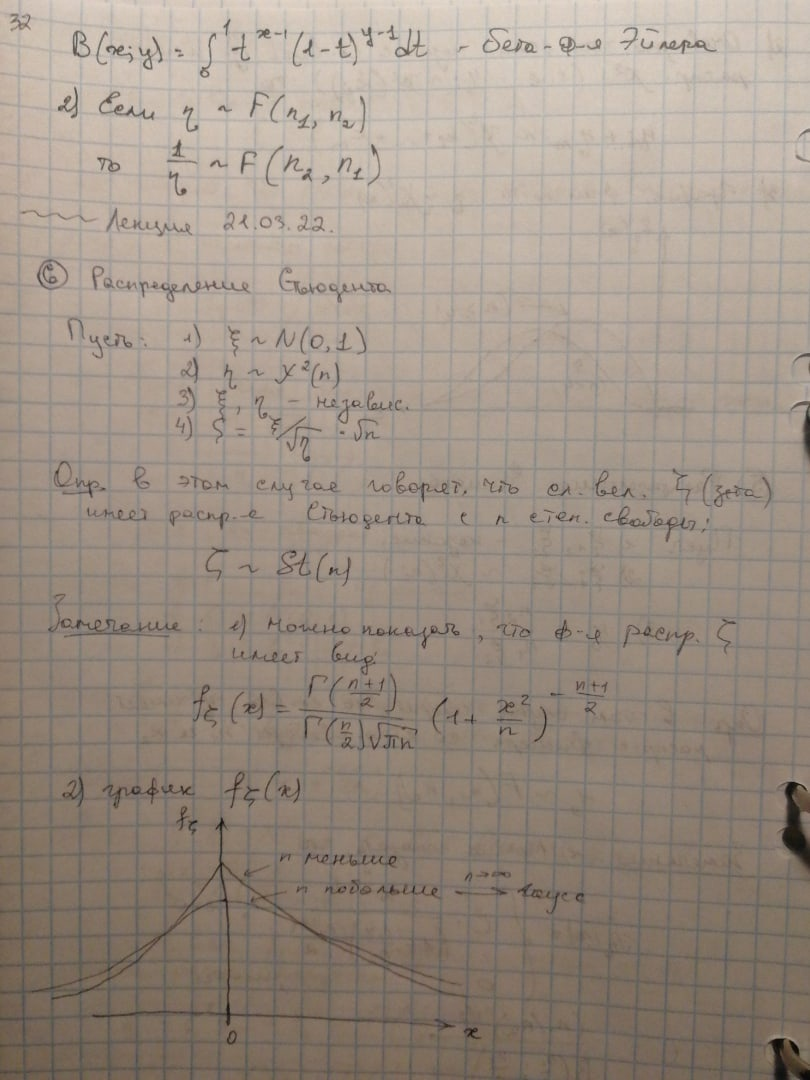
\includegraphics[scale=1.0]{1}}
	\caption{Пример построения схемы вычислений}
\end{figure}

\begin{figure}[H]
	\center{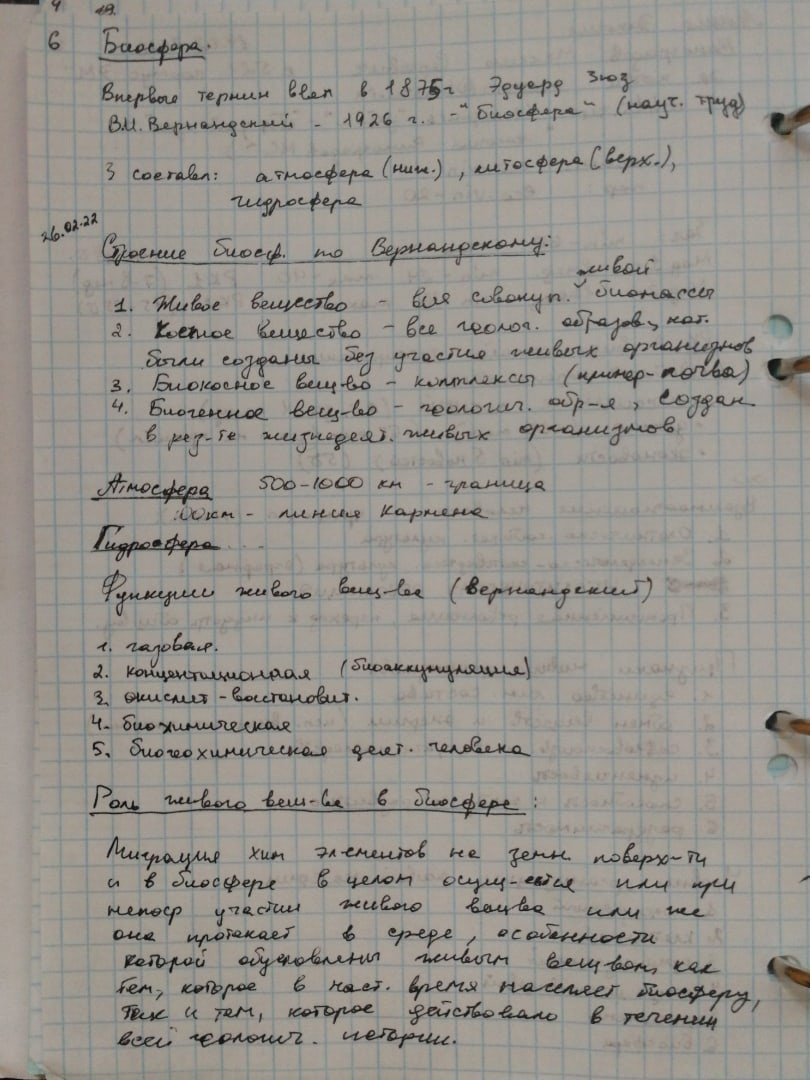
\includegraphics[scale=0.65]{2}}
	\caption{Пример построения блок-схемы работы функции}
\end{figure}

\chapter{Лекция 3}
Как функция отличает символы от функций?
Как система запоминает символы и на какое время?
Придумать метод реализации учитывая, что Lisp реализуется с помощью указателей.

\section{Функции}
Мн-во всех функций можно классифицировать:\\
1. как базисные и небазисные\\
2. по методу написания:\\
    - чистые функции имеют фиксированное количество аргументов и возвращают результат\\
    - формы - функция, которая вычисляет не все свои аргументы\\
    - функционалы - принимают на вход функцию или возвращают функцию в качестве результата\\

\section{Специальные функции}
- базисная функция (cond (test\_1 body\_1) (test\_2 body\_2) ... (test\_i body\_i) [(t body\_i+1)]), test\_i - тестирующееся выражение, body\_i - выполняется, если test\_i корректный.
- if - более удобная реализация cond, (if test than else)/(if test than) - если нет else, то автоматически возращается nil

Диаграммы во второй лабораторной.
При вызове свой функции указываются фактические параметры, в определении функции присутствуют формальные параметры. Если формальный параметр получает какое-то значение, то к этому значению необходимо иметь доступ, поэтому этому символу должна быть выделена память. Для каждого атома - 5 указателей. В процессе работы тела указатели могут переставляться и могут меняться значения, на которые указывают эти указатели. И поэтому на каждом шаге использования этого параметра система вынуждена каждый раз вычислять значение этого атома.

Формальные параметры существуют только во время работы функции -> в рекурсивной функции есть опасность потерять значение.

- логические выражения (формы and/or, not, null)

Символьному атому можно установить значение. Есть локальные атомы - существуют в фукнции, есть глобальные атомы - существуют на протяжении всей работы программы. Можно установить значение символьному атому до момента, пока это значение не поменяется. Установка происходит с помощью функций setf и setq. Эти функции имеют два аргумента, первый не вычисляется, второй вычисляется и является значением первого аргумента. Разница между setf и setq - вычисляются оба аргумента или один. 

Если в тексте программе используется установленый уникальный атом, то система использует значение установленного ранее атома. 
Список свойств - динамическая структура, состоящая из списков вида (имя свойства, свойство).

Функция let - является формой, имеет два аргумента (let ((name1 val1) (name2 val2) ... (namen valn)) body) - namen - имя указателя, valn - значение указателя namen, body - выражение, где можно использовать указатели name1 - namen. 

Работа let - сначала выделяется память, потом готовятся значения, после чего происходит связывание в произвольном порядке. При этом в name2 нельзя использовать name1, поскольку ещё не произошло связывание, поэтому при вычислении очередного значения namei нельзя ссылаться на значение предыдущих атомов.

let* - позволяет сослаться на значения предыдущих атомов, но работает менее эффективно.

\section{Функции, реализующие операции со списками}
Данные функции можно разбить на две группы - разрушающие структуру и не разрушающие структуру.

Для работы со списком его необходимо создать, получить доступ и модифицировать.

Функции, разрушающие структуру - изменяют структуру списка. Функции не разрушающую структуру - производят какие-то операции без изменения поданного на вход списка.

Функция append - функция объединяет списки. Количество аргументов может быть произвольным. Функция append работает с копией списка -> не разрушается структура списка, поданного на вход.

\begin{lstlisting}[label=some-code-2]
(setf lst1 '(a b))
(setf lst2 '(c d))

lst1 -> [][] -> [][] -> nil
        |       |
        a       b

lst1 -> [][] -> [][] -> nil
        |       |
        c       d

(setf lst3 (append lst1 lst2))

lst3 -> [][] -> [][] -> [][] -> [][] -> nil
        |       |       |       |
        a       b       c       d
\end{lstlisting}

Создаются копии списков, кроме последнего. После чего копии сцепляются последними указателями, последний прицепляется к lst2. В результате можно работать со списками lst1 и lst3, однако lst2 одновременно входит в lst3, что приводит к тому, что его изменении происходит и изменение lst3.

nconc - дубль append, nconc переставляет указатели, в результате чего списки сшиваются без создания дублей

reverse - развернуть с копиями
nreverse - развернуть без копий

last - на вход подаётся структура, состоящая из списковых ячеек, возвращает последнюю списковую ячейку.

Список может быть смешанным - числа и символы могут быть в списке. Может быть одноуровневым и многоуровневым. Структурированный/неструктурированный.

Список числовой - только из чисел.

<!> Все стандартные функции работают только с верхним уровнем списка.

(nth N lst) - n-й элемент. (nthcdr N lst) - n-й хвост. (remove elem lst) - удаление элемента, не обрабатывает внутрениие списки. 

В стандартных функциях для сравнения использует функцию equal, принимающую на вход только атомы, не списки.

member - проверка присутствия элемента в списке. (member elem lst) - по верхнему уровню ячеек, используется функци eql, не сравнивается список. Пример (member '(a, b) '(c (a b) d)) - в случае подачи, система не обнаружит, поскольку eql не сравнивает списки. Можно повлиять на работу функций с помощью механизма ключевых слов. При создании функции используется набор ключевых параметров, которые могут быть изменены для изменения поведения функции. В данном случае изменение ключевого параметра test позволит включить сравнение списков - (member '(a, b) '(c (a b) d): test \#'equal). Результат работы будет ((a b) d).

Для возврата списочных ячеек по элементу - assoc и rassel.

Работа со множествами - работа со множествами, представленными в виде списком. Существуют стандартные функции для работы с множествами. 

Ассоциативные таблицы - самый простой вариант реализации - список точечных пар, где в каждой паре точечная пара состоит из ключа и значения. Для работы с ассоциативными таблицами существует несколько стандартных функций.

\section{Функционалы}

Какие типы алгоритмов существуют? - линейный, разветвлённый, циклический.

Для организации повторных вычислений используются либо функционалы, либо рекурсии.

Функции применяющие и отображающие.

Значения глобальных атомов могут влиять на работу функции, поэтму необходимо его заблокировать. \# - функциональная блокировка, фиксирует значения глобальных атомов (фиксирует состояние в памяти окружения данной функции). \# - function - функция, вызывающая функциональную блокировку.

Функция apply - применяет лямбда-функцию к какому-либо выражению (apply \#'fun lst), fun - функция или лямбда-выражение, lst - список аргументов.
(funcall \#'fun arg1 ... argn) - применение формы, аналогично apply но без списка.

Отображающие фукнционалы - функционалы, позволяющие реализовать многократные или повторные вычисления. Результаты огранизуются в виде списка результатов для каждого вызова функции. 

Основные отображающие функционалы:
- (mapcar \#'fun lst1) - функция, указанная fun, применяется к каждому элементу списка из верхнего уровня ячеек, элементы могут быть как указателями так и списками, поэтому необходимо учитывать это при написании функции.
- (maplist \#'fun lst2) - функция применяется целиком к списку, к хвосту списка, к хвосту хвоста... пока список не станет пустым.
В данной форме функция fun должна быть одноаргументая, в функции maplist - функция fun должна уметь работать со списком.

\section{Среда}
Термин "среда" употребим, когда используется какой-то пакет. При загрузке пакета становится доступен интерфейс среды - набор возможностей, облегчающих программирование.

\chapter{Лекция 4}
\section{Функции работы со списками-}
Вызов функции mapcar для функции нескольких аргументов: (mapcar \#'fun lst1 lst2 ... lstk). В данном случае mapcar выбирает из каждого списка car аргументы и применяет их к функции. mapcar не контролирует длину списков, поданных на вход. Если списки имеют разную длину, когда заканчиваются элементы по верхнему уровню самого короткого списка.

(maplist \#'fun lst1 lst2 ... lstk), функция fun должна работать со списками.

При работе данных функций образуются несколько результатов, которые объединяются в список с помощью list. Существуют дубли, где объединение происходит с помощью функции nconc - mapcan, mapcon.

(find-if \#'fun lst) - функционал find-if проходит только по верхнему уровню списковых ячеек, возвращает первый элемент списка, удовлетворяющий данной функции (\#'fun = \#'predicat). Пример: (find-if \#'odd '(2 4 7 5)) $\rightarrow$ 7. (find-if-not \#'predicat lst) - первый элемент, fun от которого возвращает Nil.

(remove-if \#'predicat lst)/(remove-if-not \#'predicat lst) - удаление элемента с условием.

Если определение предиката написано прямо в функции, то при выполнении программы не происходит множественного перехода по указателю от имени к определению функции, поэтому данный вариант предпочтительнее, так как работает быстрее.

(reduce \#'fun lst) - каскадная функция, fun должна иметь не менее двух элементов. Сначана применяет к первым двум элементам, потом к результату и третьему, потом к результату и четвёртому.

(every \#'fun lst), (some \#'fun lst) также работают каскадным образом.

Примеры применения функционалов:\\
\begin{lstlisting}
(defun consist-of (lst)
	(if (member (car lst) (cdr lst)) 1 0))

(defun all-last-element (lst)
	(if (eql (consist-of lst) 0) (lst (car lst)) ()))

(defun collection-to-set (lst)
	(mapcon \#'all-last-element lst))

(collection-to-set '(i t i g t k s i f k))
> (g t s i f k)
\end{lstlisting}
Смысл примера - порядок результата может зависеть от порядка аргументов в исходном списке.\\

\begin{lstlisting}
(defun dcart (lstx, lsty)
	(mapcan #'(lambda (x)
		(mapcar #'(lambda (x) (list x y)) lsty))
			lstx))

(decart '(a b) '(1 2))
> ((a 1)(a 2)(b 1)(b 2))
\end{lstlisting}
Смысл примера - применение лямбда-функций и использование вложенного вызова функционала с фиксацией аргумента x.

\chapter{Лекция 5}
\section{Рекурсия}
Рекурсия - повторный вызов некой функции этой функци. Рекурсия - ссылка на некий объект в описании этого объекта. Основные вопросы при создании рекурсии - как войти, как выйти, как передать аргументы.

Классификация рекурсий в Lisp:
\begin{itemize}
\item Простая рекурсия - один вызов в теле функции
\item Рекурсия первого подярка - когда в теле функции вызов функции производится несколько раз
\item Взаимная рекурсия - в теле функции вызывается несколько разных рекурсивных функций
\end{itemize}

Первые ветки рекурсии реализуются cond - базисный случай. Золотое правило создание рекурсии - сначана проверка, нужно ли выйти из рекурсии и только потом уход на следующий шаг.

Для эффективной реализации рекурсии необходимо заранее выполнить отложенные вычисления и только затем уходить в рекурсию для того, чтобы вернуть только промежуточный результат. 

Хвостовая рекурсия - один из способов эффективной организации рекурсии.

lisp, append, cons - какую из этих функций нужно использовать, чтобы реализовать рекурсию эффективно (точно не append, поскольку append делает копии).

"Хорошая" функция - эффективность с точки зрения данных и реализации.

\begin{lstlisting}
(defun my-number (el lst)
	(cond ((null lst) Nil)
		((equal el (car lst)) t)
			(t (my-member el (cdr lst )))))

(my-member 'a (b a c))
> t
(my-member nil ())
> nil
\end{lstlisting}
В последнем вызове вывод не совсем корректный из-за порядка следования проверок cond. Переставив их местами мы можем добиться правильного вывода.

\begin{lstlisting}
(defun my-number (el lst)
	((equal el (car lst)) t)
		(cond ((null lst) Nil)
			(t (my-member el (cdr lst )))))

(my-member nil ())
> t
\end{lstlisting}

Реализация собственной функции reverse с помощью append - неэффективный способ. Данная рекурсия нехвостовая, так как результат не вычисляется на входе.
\begin{lstlisting}
(defun my-reverse (lst)
	(cond ((null lst) lst)
		(t (append (my-reverse (cdr lst))
					(cons (car lst) lst)))))
\end{lstlisting}

Реализация собственной функции reverse с помощью свой функции - эффективный способ.
\begin{lstlisting}
(defun my-reverse (lst)
	...)

(defun move-to (lst result)
	(cond ((null lst) result)
	(t (move-to (cdr lst) (cons (car lst) result)))))
\end{lstlisting}

\chapter{Лекция 6}
\section{Рекурсия}
Эффективный вариант реализации рекурсии - при входе не остаётся невыполненных команд, т.е. рекурсивный вызов последний.

Количество веток реализации рекурсии зависит от конкретной задачи.

Может быть несколько выходов из рекурсии и несколько входов в рекурсию.

Общий вид дополняемой рекурсии
\begin{lstlisting}
(defun fn (x)
	(cond (cnd-test end-value)
		(t (cons add_val(fn changed_x)))))
\end{lstlisting}

Внутри дополняемых рекурсий существует вариант дополняемой рекурсии, имеющей преобразование с условием.
\begin{lstlisting}
(defun fn (x)
	(cond (cnd-test end-value)
		(add-test add-func (fn chaged1_x))
		(t (fn changed2_x)
\end{lstlisting}

Пример:
\begin{lstlisting}
(defun extract_symbols (lst)
	(cond ((null lst) nil)
	((symbolp (car lst)
		(cons (car lst)
			(extract-symbols (cdr lst)))))))
\end{lstlisting}

Множественная рекурсия - может быть дополнительная функция, обрабатывающая два рекурсивных вызова, по голове и хвосту.

Пример:
\begin{lstlisting}
(defun cons_sells (lst)
	(if (atom lst) 0
		(+ (length lst)
			(reduce #'+
				(mapcar #'cons_sells lst)))))
\end{lstlisting}

Пример:
\begin{lstlisting}
(defun into_one_level (lst rst)
	(cond ((null lst) rst0
		((atom lst) (cons lst rst))
		(t (into_one_lecel (car lst)
					(into_one_lecel (cdr lst) rst))))))
\end{lstlisting}

boundp - связь атома со значением, fboundp - связь атома с функционалом. Свойства - упорядоченный список чётного количества элементов. putprop - назначение свойства. remprop, symb-plist.

Механизм ключевых слов:\\
\&optional - не указанный параметр, если не введён, то заменяется на nil.\\
\&rest
Пример:
\begin{lstlisting}
(defun f1 (x &optional y) (list x y))
\end{lstlisting}

\chapter{Лекция 6}
\section{Предпосылки появления Prolog}
Процесс совершенствования техники застопорился из-за отсутсвия новой элементной базы. Пролог - реализация логики предикатов в виде языка программирования. При доказательстве теорем не используются данные в привычном смысле слова.

Пролог работает со знаниями. 

Основной элемент математический логики - высказывание, которое может быть либо истинно либо ложно. 

Задача пролога - автоматизировать процесс доказательства теорем. Для решения данной задачи необходимо было доказаь принцип резолюции. Данный принцип был доказан в 1969 году. Позволяет сделать обоснованный вывод из утверждения. 

Пролог поддерживает декларативный способ программирования.

Всё что нужно для функционирования исскуственного интеллекта - обладание знаниями.

\section{Prolog}
Программа на прологе представляет из себя базу знаний. Данная база состоит из аксиом (фактов) и теорем. База знаний фиксируется в разделе, имеющем заголовок clauses - предложениия. Активизация производится в разделе go (цель).

Единственная конструкция пролога - term, либо константа, либо переменная, либо составной терм. Логическая система возвращает либо да либо нет и попутно информация о том, как дойти для нужного результата.

Основная единица - символьный атом, использующегося для обозначения предикатов. С маленькой буквы - константа, с большой буквы - переменная.

Строковые константы - в кавычках. Именованные переменные - переменные использующие имена. Prolog использует анонимные переменные, обозначающиеся как \_.

Составные термы используются для того, чтобы зафиксировать, что между какими-то объектами есть связь. F(t1, t2, ..., tn), F - главный функтор, t1-tn - термы.

Пример:\\
student(ivanov, mgtu). - конкретный студент конкретного вуза\\
student(X, mgtu). - все студенты конкретного вуза\\
student(X, Y). - все студенты всех вузов\\

Все предложения заканчиваются точкой. Количество аргументов в функторе - арность.\\
student(ivanov) - арность 1, поэтому разные знания.\\

В момент фиксации утверждение с переменной значение не имеет. Поэтому процесс работы системы заключается в том, чтобы найти решение данного предиката.

Когда система подбирает для переменной значение говорят, что система конкретизирует переменную значением. При этом при подборе система может ошибиться, поэтому система ведёт доказательство путём проб и ошибок. Работа системы - процесс доказательства, работающий на основе фактов. Активация происходит путём задания вопроса.

Синтаксическая форма правила:\\
A :- B1, B2, ..., Bk.\\ 
Факты, содержащие переменные - основные, не содержащие - неосновные. A - заголовок правила. B1-Bk - тело.\\
student(X, mgtu) :- документы(X, att), ...\\
Заголовок является фиксацией знания о том, что между аргументами возможна истинная связь (X действительно студент, если...)\\

Особенный способ работы с переменными:\\
Вместо того, чтобы сначала задавать значения переменной, задаётся условие и система ищет такие значения переменных, чтобы на вопрос ответить да. При этом сохраняюстя и возвращаются значения для этого ответа.

Переменные нужны для передачи данных во времени и пространстве.\\
Во времени - переменная получила значение и через какое-то время оно было использовано\\
В пространство - передача между областями данных (памяти) - перенос в физическом пространстве\\

Во время фиксации переменная не имеет значения.

\chapter{Лекция 7}

